\documentclass[oneside]{VUMIFPSkursinis}
\usepackage{algorithmicx}
\usepackage{algorithm}
\usepackage{algpseudocode}
\usepackage{amsfonts}
\usepackage{float}
\usepackage{amsmath}
\usepackage{bm}
\usepackage{caption}
\usepackage{color}
\usepackage{float}
\usepackage{graphicx}
\usepackage{listings}
\usepackage{subfig}
\usepackage{ltablex}
\usepackage{longtable}
\usepackage{wrapfig}
\usepackage{subfig}
\usepackage{pbox}
\renewcommand{\labelenumii}{\theenumii}
\renewcommand{\theenumii}{\theenumi.\arabic{enumii}.}
\renewcommand{\labelenumiii}{\theenumiii}
\renewcommand{\theenumiii}{\theenumii\arabic{enumiii}.}
\newcolumntype{P}[1]{>{\centering\arraybackslash}p{#1}}
\usepackage[%
	colorlinks=true,
	linkcolor=black
]{hyperref}
\university{Vilniaus universitetas}
\faculty{Matematikos ir informatikos fakultetas}
\department{Programų sistemų katedra}
\papertype{Žmogaus ir kompiuterio sąsaja laboratorinis darbas II}
\title{Alaus gamybos įrangos ir ingredientų pirkimo sistema}
\titleineng{Aludarystės internetinė parduotuvė}
\status{3 kurso studentai}
\author{Greta Pyrantaitė}
\secondauthor{Matas Savickis}
\thirdauthor{Andrius Bentkus}

\supervisor{Kristina Lapin, Doc., Dr.}
\date{Vilnius – \the\year}

\bibliography{bibliografija}

\begin{document}
\maketitle

\sectionnonum{Anotacija}
Šio darbo tikslas yra pagal pirmame laboratoriniame darbe apibrėžtus vartotojų scenarijus sukurti interfeiso maketus.
Kiekvienas komandos narys įgyvendins savo pasirinkto scenarijaus maketo idėją pasinaudodamas šabloniniais informacijos architektūros sprendimais. 
Kiti komandos nariai įvertins savo kolegos maketą parašydami savo komentarus.

\begin{itemize}
	\item{Greta Pyrantaitė - greta.pyrantaite@gmail.com}
	\item{Matas Savickis - savickis.matas@gmail.com}
	\item{Andrius Bentkus - andrius.bentkus@gmail.com}
\end{itemize}

\tableofcontents

\sectionnonum{Įvadas}
	\subsectionnonum{Programų sistemos ilgasis pavadinimas}
		Alaus gamybos įrangos ir ingredientų pirkimo sistema.
	\subsectionnonum{Programų sistemos trumpasis pavadinimas}
		Aludarystės internetinė parduotuvė
	\subsectionnonum{Dalykinė sritis}
		Elektroninė parduotuvė skirta aludariams.
	\subsectionnonum{Probleminė sritis}
		Sistema turi suteikt galimybę nusipirkti alaus gamybai reikalingus ingredientus ir įrangą bei gauti visą reikalingą informaciją apie ingredientų ir įrangos specifikacijas.
		Sistema taip pat turi vartotojui pateikti informaciją apie alaus gamybos procesą panaudojant nusipirktus ingredientus ir įrangą.
	\subsectionnonum{Naudotojai}
		\begin{itemize}
			\item{Pirkėjas(aludaris) - pirkėjas turi galėti užsisakyti alaus gamybos ingridientus ir įrangą bei gauti reikalingą specifikaciją norint naudotis preke.
				Pirkėjui turi užtekti mokyklinio informatikos kurso žinių ir bendro supratimo, kaip naviguotis internetinėse svetainėse.}
			\item{Pardavėjas - pardavėjui sistema turi suteikti informaciją apie užsakymus, jų apmokėjimus ir panašią svarbią informaciją.
				Sistema pardavėjui taip pat turi suteikti galimybę pridėti arba išimti prekes iš internetinės parduotuvės.
				Pardavėjui taip pat turi užtekti mokyklinio lygio informatikos žinių ir bendrų žinių naviguotis interneto svetainėse.}
		\end{itemize}
	\subsectionnonum{Naudoti dokumentai}
		Kristina Lapin - Žmogaus ir kompiuterio sąveikos paskaitų skaidrės, laboratorinių darbų aprašymai.


\section{Andriaus Bentkaus maketas}
	Makete yra pavaizduoti du scenarijai - pradedančio aludario pirmas užsakymas ir patyrusio aludario prekių ieškojimas.
	Pagrindinis langas šone turi pasirinkimo katalogą.
	Šalia yra atvaizduojamos prekių nuotraukos naujovėm bei populiariom prekėm ir dviem populiariausiom kategorijom.
	Produktų aprašymai yra sąmoningai nerodomi, tam kad vartotojas galėtu paįvarinti pasirinkimo metodiką ir išsirinkti produktą neskaitant jo aprašą bei kainą.
	Toks pasirinkimo būdas leidžia lengviau atrast naujas prekes, nes vartotojas nebėra bauginamas kainos bei savo nusistatymų. \newline
	Vartotojas gali pasirinkti prekę tiesiogiai arba per kategorijų menių per kategorijos, taip pat per atvaizduojamas populiariausias kategorijas.
	Vartotojui pasirinkus bendrą kategoriją arba subkategorija prekės yra atvaizduojamos iškarto su nuotrauka bei svarbiausiais atributais ir kaina.
	Po prekės nuotrauka, jos svarbiausių specifikacijų aprašą bei kainą yra mygtukas Į krepšelį", kuris įdeda prekę į krepšelį, visur kitur prekės keturkampyje spragtelėjus mygtuką atidaromas detalus prekės aprašymas. \newline
	Detaliam aprašyme yra pavaizduojama pagrindine nuotrauka bei alternatyvios mažesniu formatu po ja - paspaudus mažesnes, pagrindinė nuotrauka pakeičiama į paspaustos nuotraukos vaizda.
	Be svarbiausių prekės rodiklių dar yra pavaizduojamas detalus aprašymas bei pasiūlomos panašios prekės po detalaus aprašymo. \newline
	Vartotojui paspaudus "Kaip pasigaminti" menių skiltį jis yra nuvedamas į puslapį su alaus gamybos instrukcija pradedantiesiam.
	Instrukcijoje yra video instruktažas bei detalus aprašymas tekstu kaip pasigaminti alų.
	Kiekvienojė eilutėje kur yra paminėta prekė tam pačiam lygyje dešinėje dar yra mygtukas, kuris leidžia paminėtą prekę įsidėti į krepšelį.
	Po viso instruktažo taip pat yra mygtukas, kuris leidžia visas prekes iškarto įsidėti į krepšelį, tačiau jį paspaudūs vartotojas yra ispėjamas ispėjimo lange, jog būs pridėta daugiau negu viena prekė.

	\subsection{Mato Savickio komentaras}
Maketas atrodo tvarkingas ir simplistiškas. Įdomus sprendimas buvo pagrindiniame lange prekes rodyti tik paveiksliukais. Prekių saraše taip pat aiškiai pateiktas trumpas prekės aprašymas kuris padės lengviau surasti norimą prekę. Galbūt bus šiek tiek sunkiau najiems vartotojams tik atėjus į puslapį matyti tiesiog paveiksliukus ir bus sunkiau susikoncentruoti ir pamatyti ,,Kaip pasigaminti" mygtuką.
	\subsection{Gretos Pyrantaitės komentaras}

\section{Gretos Pyrantaitės maketas}
\begin{figure}
  		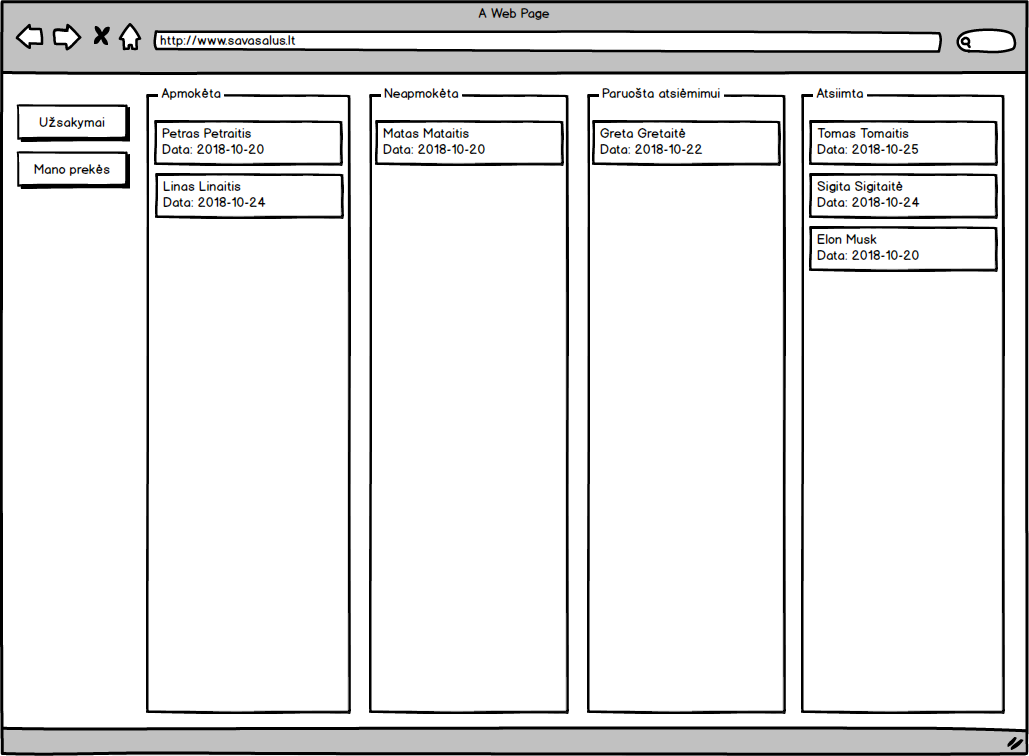
\includegraphics[width=\linewidth]{Mano_uzsakymai.png}
  		\caption{Pagrindinis maketo langas}
 		 \label{fig:mak2}
	\end{figure}
Mano maketai apima pardavėjo scenarijus -  būtent pardavėjo užsakymų peržiūra bei prekės išimimas iš prekybos.
Pagrindinio lango maketas padarytas navigacijos pasirinkimo pagrindu ir dalykinio turinio klasifikacija, kur išskirtos atskiros dalys pagal užsakymo būseną: apmokėta, neapmokėta, paruošta atsiėmimui, atsiimta. 
Taip patogiau pardavėjui gaudytis, į kuriuos užsakymus kreipti dėmesį.
Paspaudus ant užsakymo, šalia parodoma daugiau informacijos apie užsakovą, užsakytas prekes, taip pat yra galimybė arba pakeisti užsakymo būseną, arba jį atšaukti.
Pardavėjui norint peržiūrėti jo į parduotuvę įkeltas prekes, atsiveria langas su prekių sąrašu.
Taip pat, navigacijos meniu šalia mygtuko ''Mano prekės'' atsiranda mygtukai, kurie suskirsto prekes pagal tipą, jei atsirastų poreikis peržiūrėti tik tam tikro tipo prekes.
Paspaudus prie prekės mygtuką ''Peržiūrėti'' atsiveria langas su daugiau informacijos apie pasirinktą prekę.
Visus langus galima redaguoti, o norint pašalinti prekę iš prekybos reikia patvirtinti pasirinkimą pasirinkimo lange.
Maketai sukurti norint palengvinti ir pagreitinti pardavėjo navigaciją užsakymuose ir prekėse tuo pačiu užtikrinant, kad neįvyktų atsitiktinės klaidos.

	
	\subsection{Andriaus Bentkaus komentaras}
	\subsection{Mato Savickio komentaras}
Užsakymų langas padarytas įdomiu Kamban stiliumi, pardavėjui visi užsakymai sugrupuoti aiškiai, akis gali susikoncentruoti ties viena iš grupių. Šioje dalyje galbūt norėtūsi sukeisti vietomis Apmokėtus su Neapmokėtais užsakymus, nes struktūra būtų šiek tiek logiškesnė, iš pradžių užsisakai, bet pamiršti apmokėti, tada apmoki, tuomet tau būna paruošiama prakė kol galiausiai ją atsiimi. Visas užsakymo veiksmas vyktų iš kairės į dešinę. Užsakymo informacijos lange vietoj ,,drop down"  sąrašo labiau tiktų ,,radio button" tai sumažintų reikalingų paspaudimų kiekį norint pakeisti būseną. Bendrai maketas yra aiškus, konkretus ir deramas pardėjui, kuriam svarbiau aiški ir detali informacija.

\section{Mato Savickio maketas}
	\begin{figure}
  		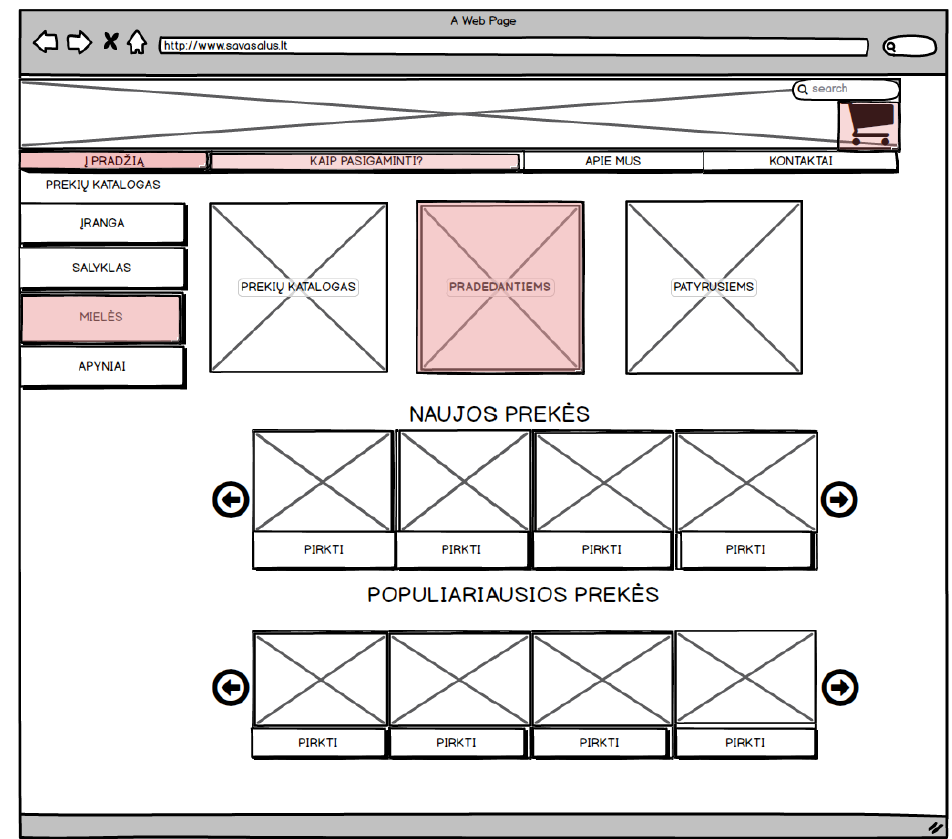
\includegraphics[width=\linewidth]{mak1.png}
  		\caption{Pagrindinis maketo langas}
 		 \label{fig:mak1}
	\end{figure}

Mano sukurto maketo pagrindinis langas susideda iš dviejų informacijos architektūros praktikų: navigacijos pasirinkimo pagrindu ir navigavimas pasirenkant. 
Mano pasirinkti scenarijai aprašė naujo vartotojo scenarijų internetinėje parduotuvėje. 
Navigacija pasirinkimo pagrindu buvo pateikta viršutinėje navigacijos juostoje, kurioje kairėje pusėje yra mygtukas ,,KAIP PASIGAMINTI?", o dvimatis navigavimas pateiktas trimis paveikslėliais iš karto po meniu juostos, o vidurinis paveikliukas yra ,,PRADEDANTIEMS". 
Nutariau, kad tą patį funkcionalumą reikia pakartoti du kartus dėl to, kad naujas vartotojas kuo greičiau pamatytų ir pasinaudotų šiuo funkcionalumu ir greičiau pradėtų naudotis parduotuve. 
Pasirinkus pradedančiojo skirtį vartotojas nukeliamas į naują puslapį, kuriame automatiškai įsijungia vaizdo įrašas, demonstruojantis, kaip pasigaminti alų. 
Instrukcijos glaustu formatu taip pat pateikiamos po video langu, o iš kairės pusės yra išrikiuotos prekės naudojamos video gaminant alų.
Vartotojas gali pasirinkti arba pridėti prekes po vieną arba pirkti visas prekes kartu. 
Vartotojui pasirikus ,,Pirkti visas prekes" jis yra nukeliamas į prekių krepšelį, kuriame gali pašalinti prekę arba atsiskaityti. 
Pasirinkus atsiskaityti vartotojas nukeliamas į atsiskaitymo langą, kuriame jis pateikia savo informaciją. 
Svarbus šio lango aspektas yra tai, kad vartotojui nebūtnai registruotis, kas pagreitina pirkimo procesą. 
Vartotojo patirtį pagerina ir tai, kad vedant skirtingą atsiskaitymo informaciją puslapis nepersikrauna.
 Užpildžius pristatymo informaciją, atsiėmimo būdą ir patvirtinus užsakymą, vartotojui parodomas sėkmingo pirkimo pranešimas. \newline
Antras scenarijus buvo vartotojo nepatogumas renkantis prekę.
Vartotojui kairėje pusėje paspaudus ant meniu pasirinkimo puslapis persikraudavo.
Savo makete pavaizduoju, kad vartotojui pasirinkus ,,Mielės" sumuštinio principu pasirodo mielių subkategorijos ir tik pasirinkus vieną iš subkategorijų puslapis persikrauna ir parodomos prekės.
	\subsection{Gretos Pyrantaitės komentaras}
	Maketas švarus, nėra per daug pasirinkimų ar nereikalingų mygtukų. Ypatingai gerai atrodo pagrindinis langas, nes pirkėjui iškart pasiūloma suskirstyti prekes pagal patyrimo lygį aludarystėje.
	\subsection{Andriaus Bentkaus komentaras}

\end{document}
